\documentclass[a4paper,11pt]{article}
\usepackage[utf8]{inputenc}
\usepackage[T1]{fontenc}
\usepackage{amsmath}
\usepackage{mathtools}
\usepackage{amsfonts}
\usepackage{amssymb}
\usepackage{graphicx}
\usepackage{multicol}
\usepackage{array}
\usepackage{float}
\usepackage{epstopdf}
\usepackage{caption}
\usepackage{subcaption}
\usepackage{gensymb}
\usepackage[bottom]{footmisc}
\usepackage{appendix}
\usepackage{pdfpages}
\usepackage{todonotes}
\usepackage{mathpazo}
\usepackage{titleps}
\usepackage{color}
\usepackage{xcolor}
\usepackage{colortbl}
\usepackage{siunitx}
\usepackage{pdflscape}
\usepackage{cancel}

\usepackage[skins]{tcolorbox}
\usepackage{sectsty}
\usepackage[arrowmos]{circuitikz}
\usepackage{pgfplots}
\usepackage{blindtext}
\usepackage[inner=2cm,outer=2cm,top=2.5cm,bottom=2.5cm]{geometry}
\usepackage{todonotes}
\usepackage{hyperref}
\usepackage{url}
\usepackage{adjustbox}
\usepackage{tabularx}
\usepackage{booktabs}
\usepackage{fancybox}
\usepackage[tikz]{bclogo}

\graphicspath{{figs/}}
\sectionfont{\large}
\subsectionfont{\normalsize}

%%%%%%%%%%%%%%%%%%%
% HANDS-ON NUMBER
% \newcommand\handsOnN{2a}
% WEEK NUMBER
\newcommand\weekN{2}
%%%%%%%%%%%%%%%%%%%

\newpagestyle{main}{
	\sethead[LELEC2102: Guide - how to use the boards][][]{LELEC2102: how to use the boards}{}{}
	\headrule
    \setfoot[][\thepage][]{}{\thepage}{}
}

\newcommand{\horrule}[1]{\rule{\linewidth}{#1}} % Create horizontal rule command with 1 argument of height

%%%%%%%%%%%%%%%%%%%%%%%%%%%%%%%%%%%%%%%%%%%%%%%%%%%%%%%%%%%%%%%%%%%%%%%%%%%%

\begin{document}
\renewcommand{\figurename}{Fig.}

\renewcommand{\thepage}{\arabic{page}}
\setcounter{page}{1}
\pagestyle{main}
\newpage \clearpage

\begin{center}
\begin{huge}
Guide: how to use the boards\\
\end{huge}
\vspace{0.3cm}
%\textit{TA 1, TA 2}
\end{center}

\section*{Introduction}

In this hands-on, you will learn how to demodulate wireless transmissions using a software-defined radio (SDR).
In the final application, the S2LP radio of the MCU transmits to a gateway that embeds an FSK receiver.
This receiver runs in GNU Radio and uses the LimeSDR Mini, a SDR board, to recover the
baseband samples of the transmitted packet. The received samples are demodulated using the open source SDR \href{https://wiki.gnuradio.org/index.php/Main_Page}{GNU Radio software}.
To this end, the teaching team developed a full GNU Radio implementation\footnote{At the exception of the demodulation and CFO estimation functions that you wrote previously.}
of a FSK receiver compatible with the S2LP radio used in the project.
The main objective of this hands-on is to experimentally receive packets from the S2LP radio and to demodulate them in GNU Radio.

\section*{Objectives}

\begin{itemize}
    \item Discover the Nucleo MCU board and its programming tools ;
    \item Learn the basics of bare metal embedded programming, General-Purpose Inputs-Outputs (GPIOs), interrupts and timers ;
    \item Understand qualitatively and measure quantitatively how the embedded software program impacts the MCU power consumption ;
    \item Learn how to debug an embedded program by logging/tracing and using a physical debugger.
\end{itemize}

\section*{Material}

\begin{comment}[couleur = gray!20, arrondi = 0.2, logo=\bcinfo]{}
\vspace{0.2cm}
\end{comment}
For this hands-on session, you will need:
\begin{itemize}
    \item The latest version of STM32 Cube IDE installed on your host system (for further information, see INSTALL.md on the GitHub of the course) ;
    \item The Nucleo MCU board with its sensing and power-management board ;
    \item A USB cable to connect your computer to the Nucleo.
\end{itemize}
%\vspace{0.01cm}

\clearpage
\section{Overview of the sensing and power-management custom board} \label{sec:custom}

This section helps you to better understand the different blocks present on the \texttt{sensing and power management} board and how you can use it throughout this project. Figure \ref{fig:pcb-overview} gives a simplified overview of the custom board while the full schematic is given in Fig \ref{fig:schematic}. Please do not try to figure out how it works without having read carefully this guide beforehand. \\

You will not need to master all parts of this board for the first weeks, but it is important that you get aware of the functionalities available on the board and what to be careful with. A good practice to keep in mind is to \textit{never} power a system (i.e. a board, a test setup or whatever) if you have not checked in advance that everything seemed to be properly connected and set. Having a quick visual check and being focused on what you are doing is critical not to damage the hardware.

\begin{figure}[h!]
    \centering
    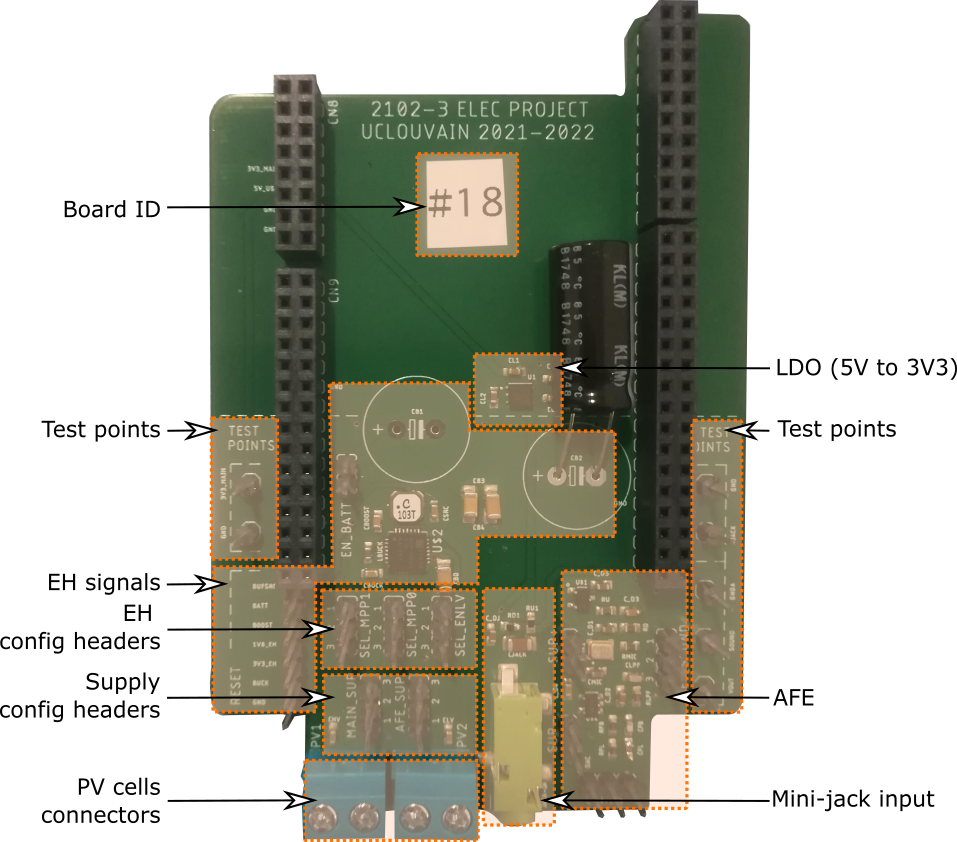
\includegraphics[width=0.8\textwidth]{figs/pcb-overview.png}
    \caption{Simplified overview of the \texttt{sensing and power-management} board, block by block.}
    \label{fig:pcb-overview}
\end{figure}

\clearpage
\subsection{Test points}

These headers allow you to monitor several useful signals on the board. Typically, you have easy access to the following signals:

\begin{table}[h!]
    \centering
    \begin{tabular}{l l }
         \textbf{Header} & \textbf{Description} \\
         \toprule
         3V3\_MAIN & Main power supply of the boards \\
                   & It supplies also the MCU on the \texttt{STM32 NUCLEO} MCU board  \\
         GND & Ground \\
         JACK & Signal at the output of the HPF, after the mini-jack \\
         SOUND & Signal sent to the ADC on the \texttt{STM32 NUCLEO} MCU board \\
         VOUT & Signal at the output of the amplifier (before the LPF) \\
    \end{tabular}
    \caption{Test points signals}
    \label{tab:TP-signals}
\end{table}

\subsection{EH signals}

These headers allow you to monitor EH signals on the board. Typically, you have easy access to the following signals:

\begin{table}[h!]
    \centering
    \begin{tabular}{l l }
         \textbf{Header} & \textbf{Description} \\
         \toprule
         BUFSRC & Voltage on the BUFSRC node \\
         BATT & Voltage on the storage capacitor(s) \\
         BOOST & Voltage on the BOOST node \\
         1V8\_EH & LVOUT output \\
         3V3\_EH & HVOUT output \\
         BUCK & Voltage on the BUCK node \\
         GND & Ground
    \end{tabular}
    \caption{Test points signals}
    \label{tab:TP-signals}
\end{table}

By default, a $150 \mu F$ capacitor is used as storing device for the EH part. To this minimum, additional storage devices can be added as shown in the schematic of the board in Fig. \ref{fig:schematic} (not all of them have be soldered on the board yet). To connect these supplementary capacitors, connect the EN\_BATT jumper.

\subsection{EH config headers}

These headers allow you to configure the EH part of the board as described in Table \ref{tab:EH-headers}. Please refer to the AEM10941 datasheet for more details about the maximum power point (MPP) tracking configuration and the outputs available (\url{https://www.mouser.be/datasheet/2/1087/e_peas_AEM10941_datasheet_energy_harvesting-2325372.pdf}).

\begin{table}[h!]
    \centering
    \begin{tabular}{l c l}
         \textbf{Header} & \textbf{Config: Jumper on Pin 2 + Pin\dots} & \textbf{Description} \\
         \toprule
         SEL\_MPP0 (2) & 1 & Tied down, i.e. GND = 0 V  \\
                       & 3 & Tied up, i.e. BUCK = 3.3 V \\
         SEL\_MPP1 (2) & 1 & Tied down, i.e. GND = 0 V  \\
                       & 3 & Tied up, i.e. BUCK = 3.3 V \\
         SEL\_ENLV (2) & 1 & LVOUT disabled \\
                       & 3 & LVOUT enabled (1.8 V)\\
    \end{tabular}
    \caption{Available configurations for the EH headers}
    \label{tab:EH-headers}
\end{table}

\subsection{Supply config headers}

These headers allow you to configure the supplies (of the boards and AFE parts) as described in Table \ref{tab:supply-headers}.

\begin{table}[h!]
    \centering
    \begin{tabular}{l >{\centering}p{8em} l}
         \textbf{Header} & \textbf{Config: Jumper on Pin 2 + Pin\dots} & \textbf{Description} \\
         \toprule
         MAIN\_SUP (2) & 1 & Select the 3V3\_EH source as the main power supply \\
                   & 3 & Select the 3V3\_USB source as the main power supply \\
         AFE\_SUP (2) & 1 & Select the 1V8\_EH as power supply for the AFE  \\
                   & 3 & Select the 3V3\_MAIN source as power supply for the AFE \\
    \end{tabular}
    \caption{Available configurations for the supply headers}
    \label{tab:supply-headers}
\end{table}

\subsection{AFE}

The schematic of the AFE can be found in Fig. \ref{fig:schematic}. The annotations provided on this figure should help you to better understand the function of each part of the circuit. Feel free to zoom-in to see details properly ! Useful datasheets for specific components are also provided on the Moodle in the folder \texttt{Technical resources}. \\

The frequency response of the AFE simulated in LTSpice is provided in Fig. \ref{fig:bode_AFE}. $V_{VOUT}$ and $V_{LP}$ are respectively the output of the amplifier and the output of the additional low pass filter, as shown in Fig. \ref{fig:schematic}. \\

In order to enable the AFE part on the custom board, you must connect the jumpers SUP+ and SUP-. The SEL\_SOUND header can be used to configure which signal you send to the ADC of the MCU, as described in Table \ref{tab:afe-headers}.

\begin{table}[h!]
    \centering
    \begin{tabular}{l >{\centering}p{8em} p{0.5\textwidth}}
         \textbf{Header} & \textbf{Config: Jumper on Pin 2 + Pin\dots} & \textbf{Description} \\
         \toprule
         SEL\_SOUND (2) & 1 & Select the JACK signal as the input for the ADC \\
                   & 3 & Select the output of the LPF signal of the AFE as the input for the ADC
    \end{tabular}
    \caption{Available configurations for the supply headers}
    \label{tab:afe-headers}
\end{table}

The CTRLS headers are currently not used in the design of the AFE. Consequently, they have no impact on the AFE behavior. However, keep in mind that in these three headers, one is a DAC and the two other ones are GPIO connections to the MCU. That might be useful in the second part of the project (LELEC2103) if you want to design a custom AFE.



% \begin{figure}[h!]
%     \centering
%     \includegraphics[width=1\textwidth]{figs/afe.png}
%     \caption{Analog Front-End (AFE) schematic.}
%     \label{fig:afe}
% \end{figure}

\clearpage
\begin{figure}[h!]
    \centering
    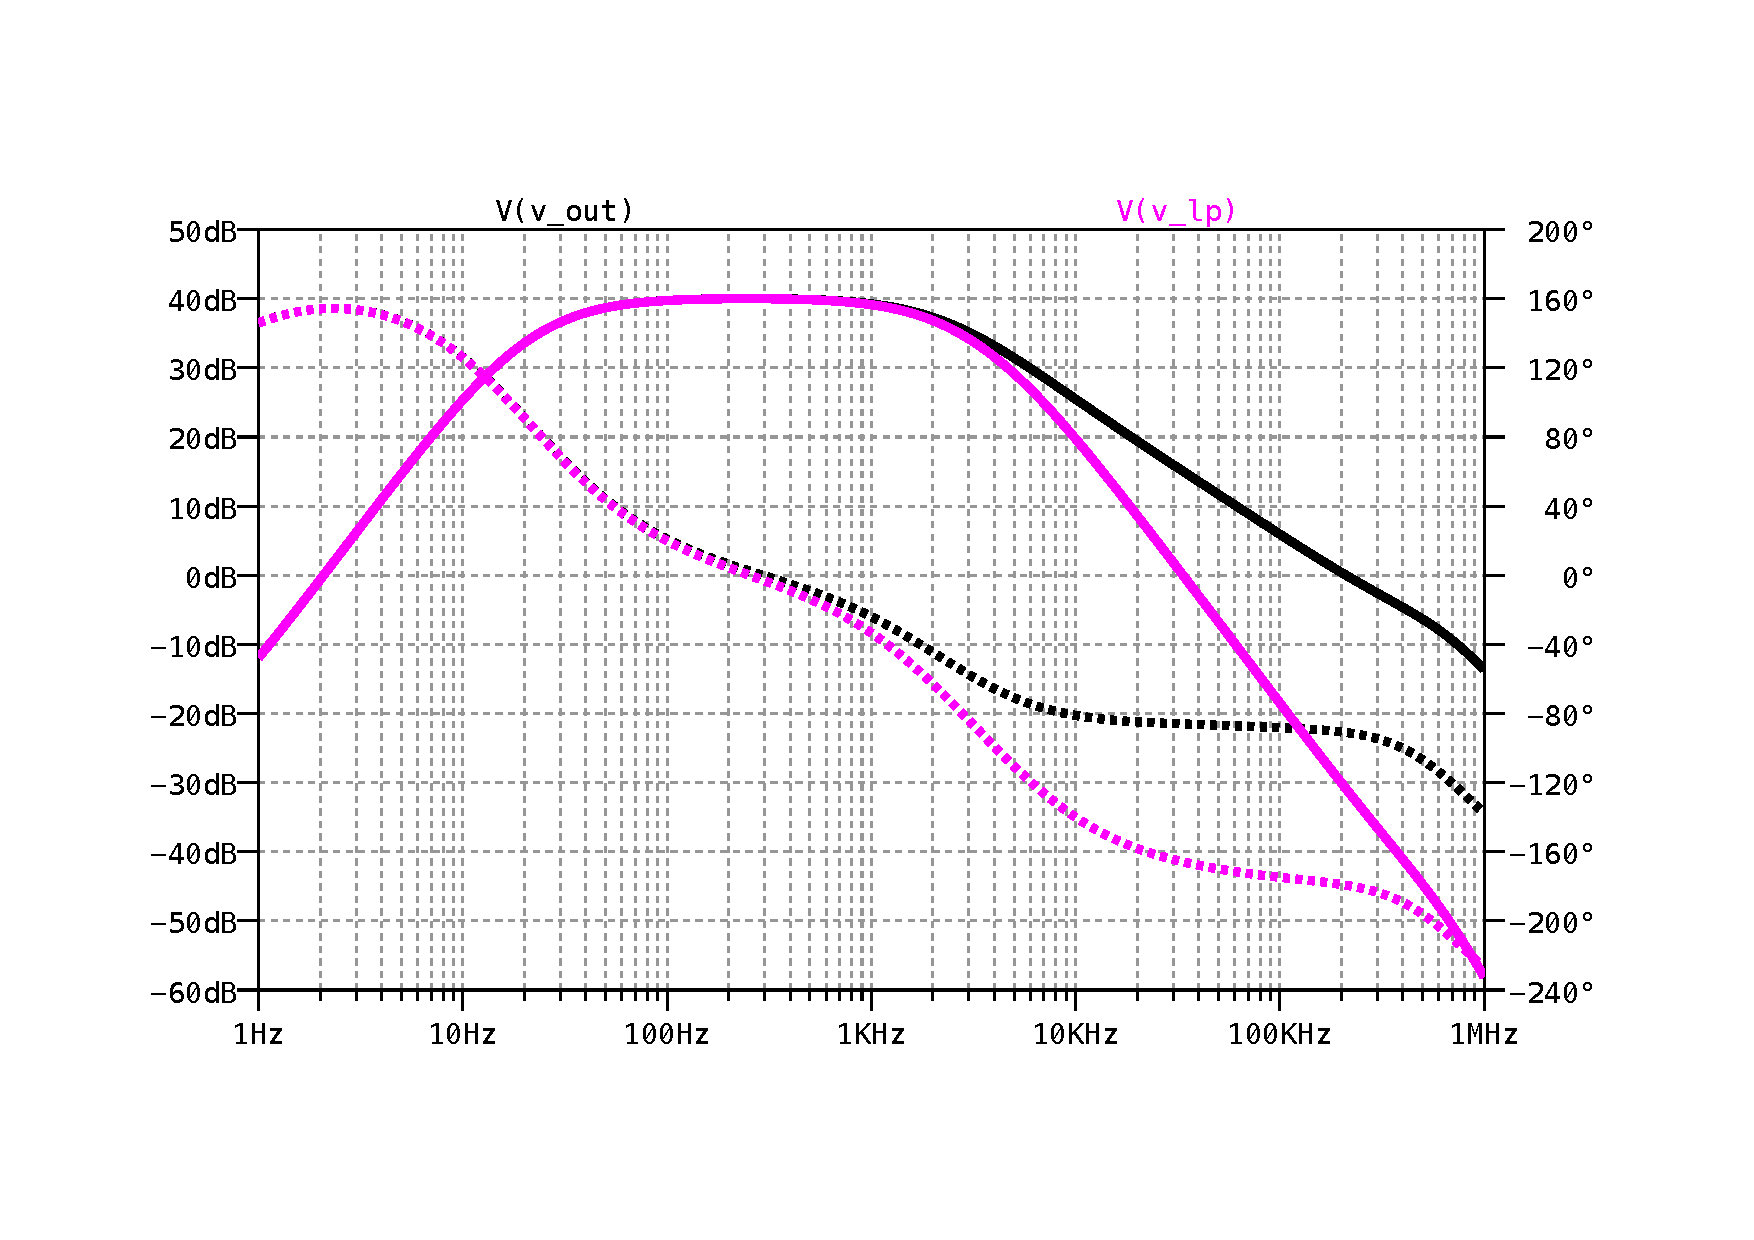
\includegraphics[scale=0.8, angle=90]{figs/bode_AFE.pdf}
    \caption{LTSpice results for the simulation of the AFE. Note: the microphone is not modeled in this simulation. The LTSpice model provided by Microchip has been used for the MCP6231.}
    \label{fig:bode_AFE}
\end{figure}

\clearpage
\subsection{Schematic of the sensing and power-management board}

\begin{figure}[h!]
    \centering
    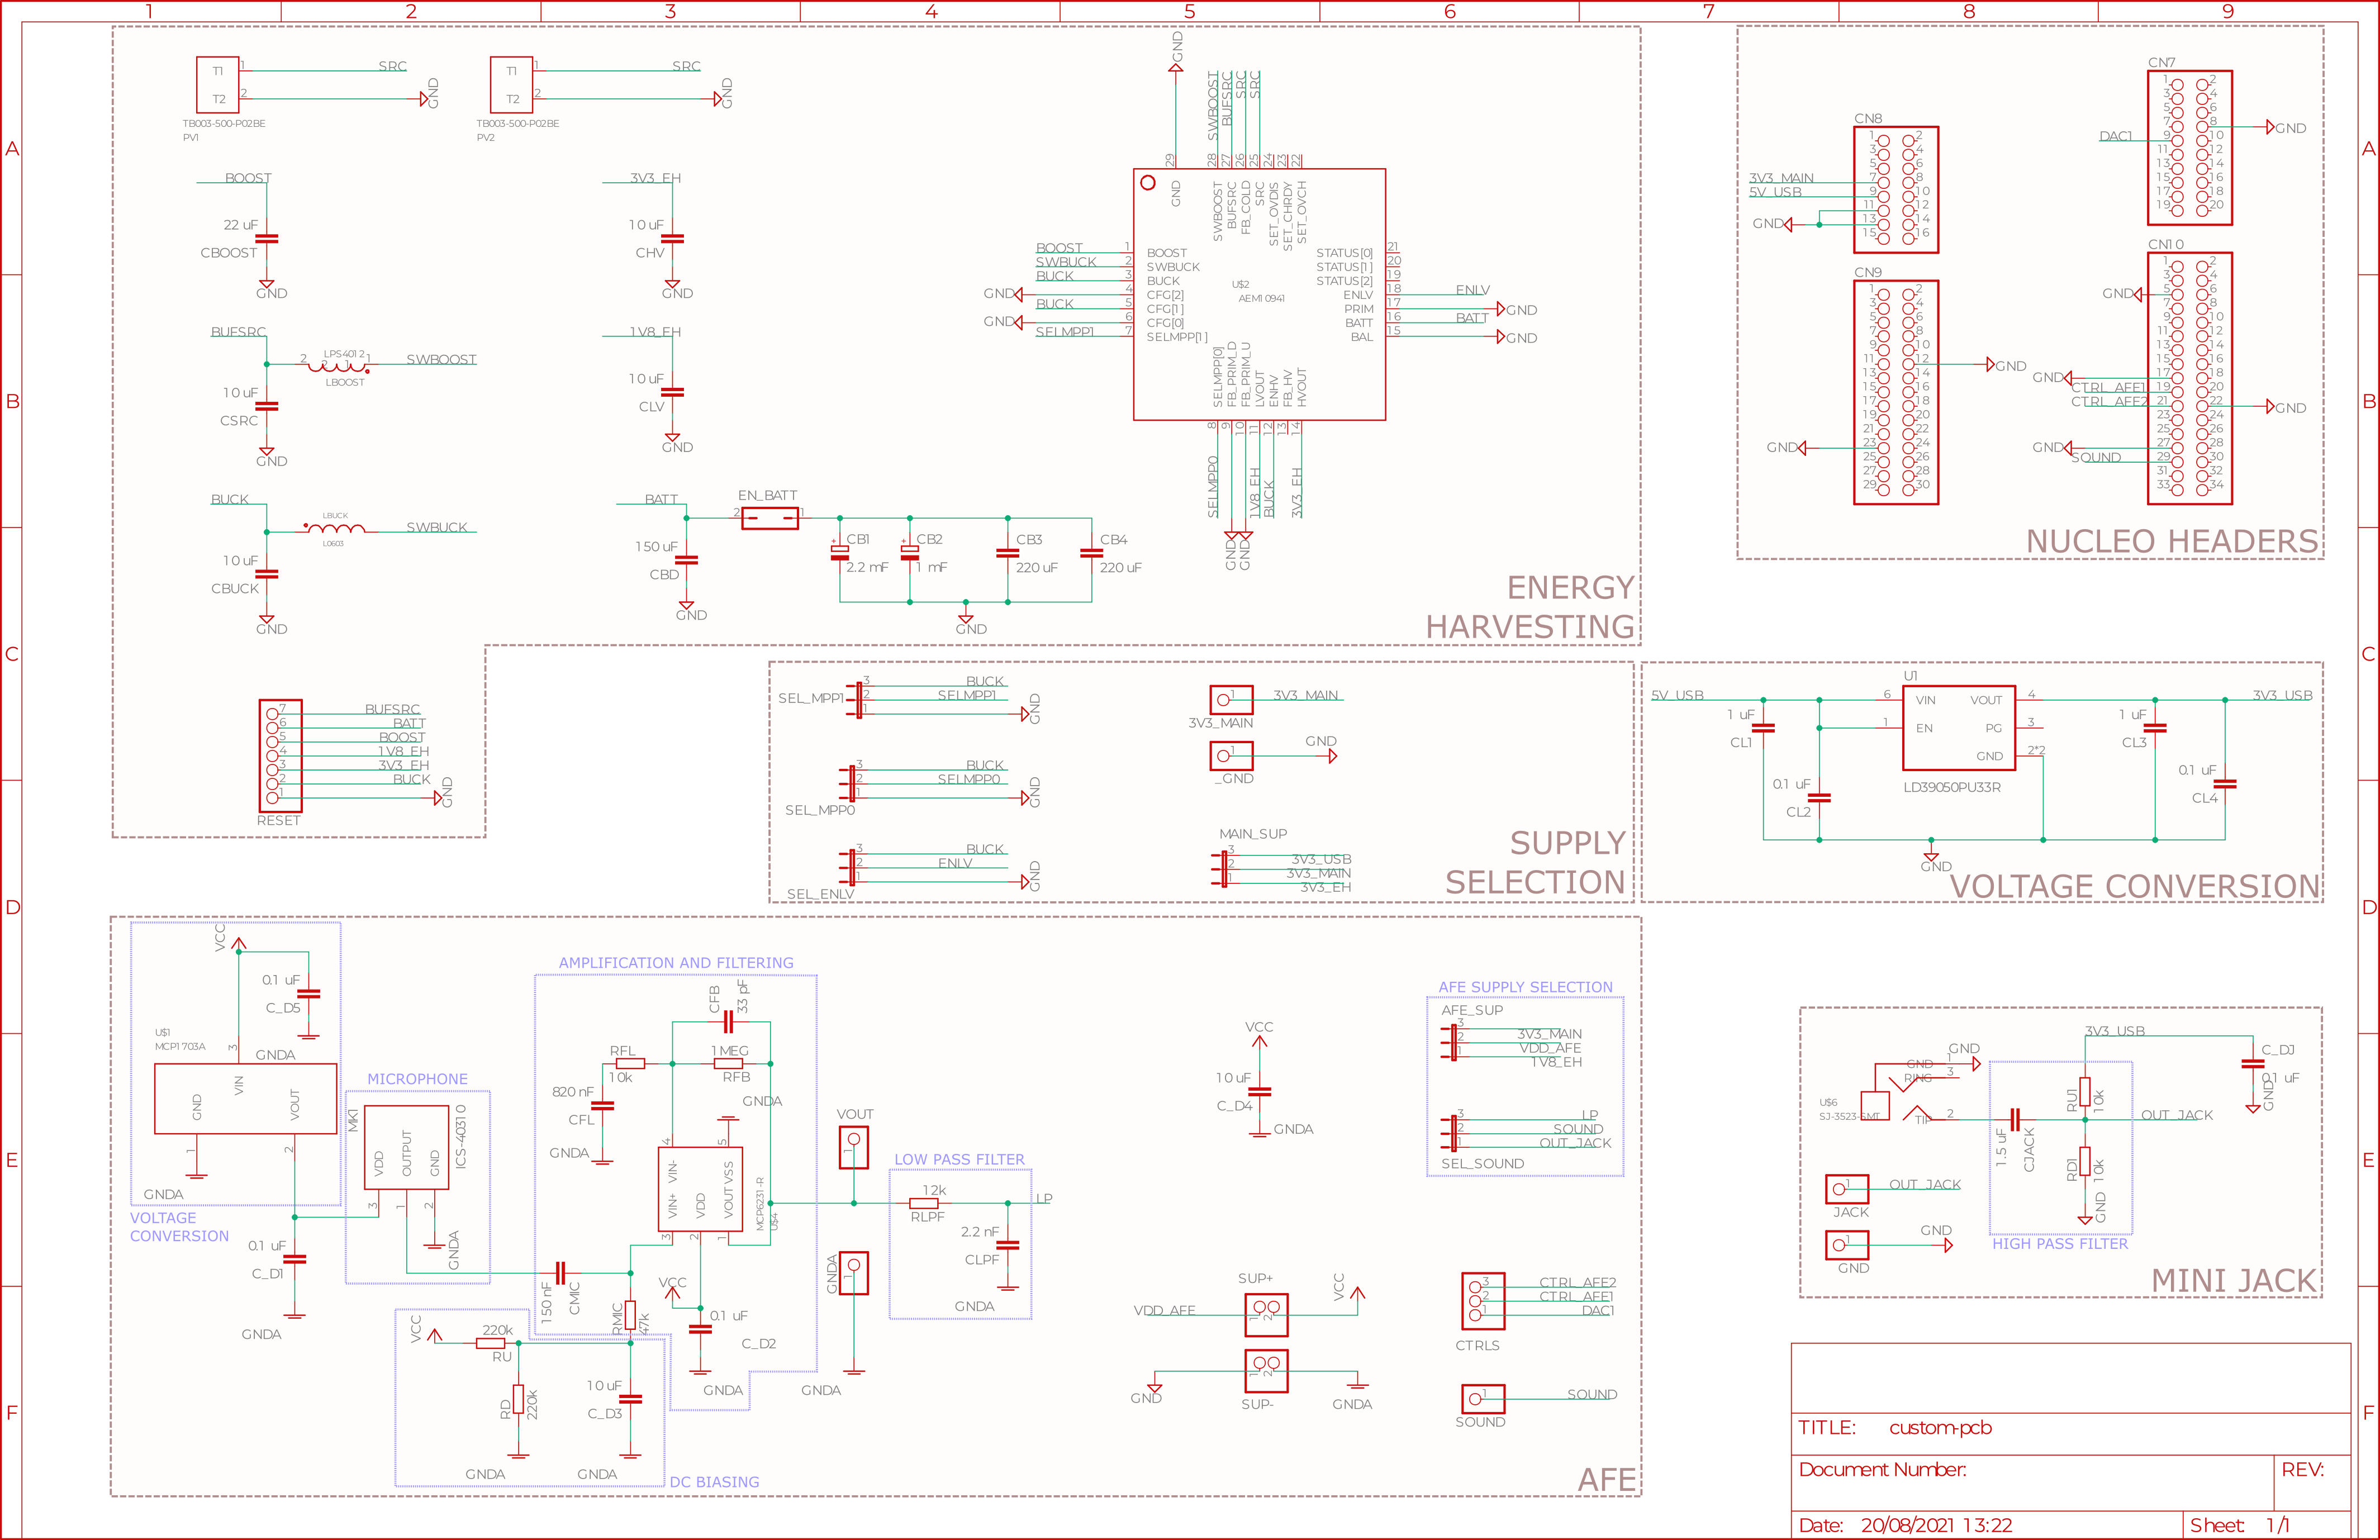
\includegraphics[scale=1, angle=90]{figs/schematic.png}
    \caption{Schematic of the \texttt{sensing and power-management} board.}
    \label{fig:schematic}
\end{figure}

\clearpage
\section{Setting the boards in the appropriate MODE} \label{sec:modes}

%%%%%%%%%%%%%%%%%%%%%%%%%%%%%%%%%%%%%%%%%%%%%%%%%%%%%%%%%%%%%%%%%%%%%%%%%%%%%%%%%%%%
\subsection{Development mode: powered by USB (ST-LINK)} \label{sec:mode-dev}

This mode is the one that you will use the most during this project. Good point, as it is the more convenient! You can basically do everything you need in this mode by simply connecting the \texttt{STM32} board to your computer through USB. It will allow you to power all the boards, program the MCU and debug it and finally receive data from the MCU through the UART interface. For this reason, it is called \textit{Development mode} as it is the one you must use to develop your project.

\textbf{In order not to damage the boards}, you need to make sure the following settings are properly set on your hardware:

\begin{itemize}
    \item First, make sure that all jumpers shown in red in Fig \ref{fig:settings-mode-dev} are configured as in the Figure. There is nothing to set on the radio board.
    \item Then, plug in your USB-micro cable as shown in Fig. \ref{fig:settings-mode-dev}. This USB port is the one to use for the ST-LINK. The USB port at the opposite of the board is an interface for the MCU but we will not use it in this project.
    \item Finally, plug in the USB-A in your computer. The "PWR LED" (yellow-green) should be ON.
\end{itemize}

\begin{figure}[h!]
    \centering
    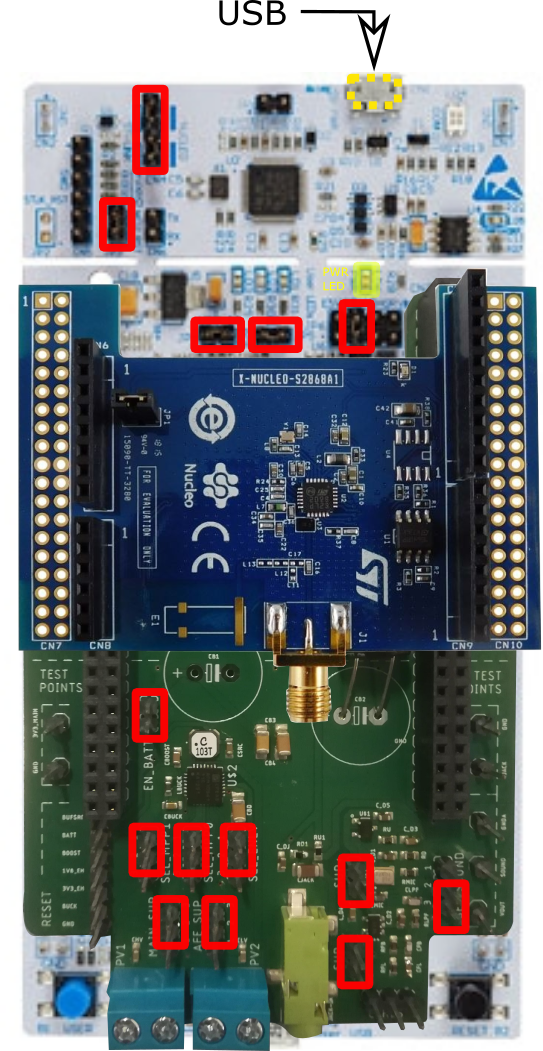
\includegraphics[width=0.4\textwidth]{figs/settings-mode-dev.png}
    \caption{Settings for the boards, development mode.}
    \label{fig:settings-mode-dev}
\end{figure}

%%%%%%%%%%%%%%%%%%%%%%%%%%%%%%%%%%%%%%%%%%%%%%%%%%%%%%%%%%%%%%%%%%%%%%%%%%%%%%%%%%%%
\clearpage
\subsection{Power monitoring mode: powered by an external 3V3 source} \label{sec:mode-3V3}

This mode is the one that you will use to monitor the \textbf{total} power drawn by your wireless smart sensors. In this mode, you have a limited amount of functionalities: it allows you to power all the boards through the external 3V3 supply but you cannot program the MCU anymore (or even debug it!). It means that you must program your MCU in advance in the development mode and then switch to this mode. In this mode, you cannot receive data from the MCU through the UART interface either. As you might guess, this is therefore not the proper mode for developing your solution! The main purpose here is to monitor the total power needed by your device once you come up with something functional. Note that in the Hands-On H2a, you will learn how to monitor the power consumption of the MCU (only) by using a dedicated jumper on the \texttt{STM32L4A6 NUCLEO-144} MCU board. However, this mode allows you to monitor the overall power consumption of your node, which is critical to make sure it remains in the power budget.

\textbf{In order not to damage the boards}, you need to make sure the following settings are properly set on your hardware:

\begin{itemize}
    \item First, make sure that all jumpers shown in red in Fig \ref{fig:settings-mode-3V3} are configured as in the Figure.
    Be really careful for the OFF jumpers: these slots have to be open (with NO jumper). If you are not sure, please call us before powering the board. It is always a better idea to ask a question rather than damaging the boards. There is nothing to set on the radio board.
    \item Then, set your external power source on 3V3 and plug it in as shown in Fig. \ref{fig:settings-mode-3V3}. Note: if you can set a maximum current as limiter, you can choose 80 mA.
    \item Finally, turn on your external power source.
\end{itemize}

\begin{bclogo}[couleur = gray!20, arrondi = 0.2, logo=\bcattention]{BE CAREFUL}
Make sure the MAIN\_SUP jumper is OFF \textit{before} powering the boards with the external power supply.
\end{bclogo}

\begin{bclogo}[couleur = gray!20, arrondi = 0.2, logo=\bcinfo]{Going below 3V3}
By using the same setup as the one proposed in this section, you can supply your system with a voltage below 3V3. You can experience by yourself down to which voltage the system can still work (Note: decrease the supply voltage step-by-step and use the datasheets to have a rough idea of the functional range of key components i.e. MCU, ...).
\end{bclogo}

\begin{figure}[h!]
    \centering
    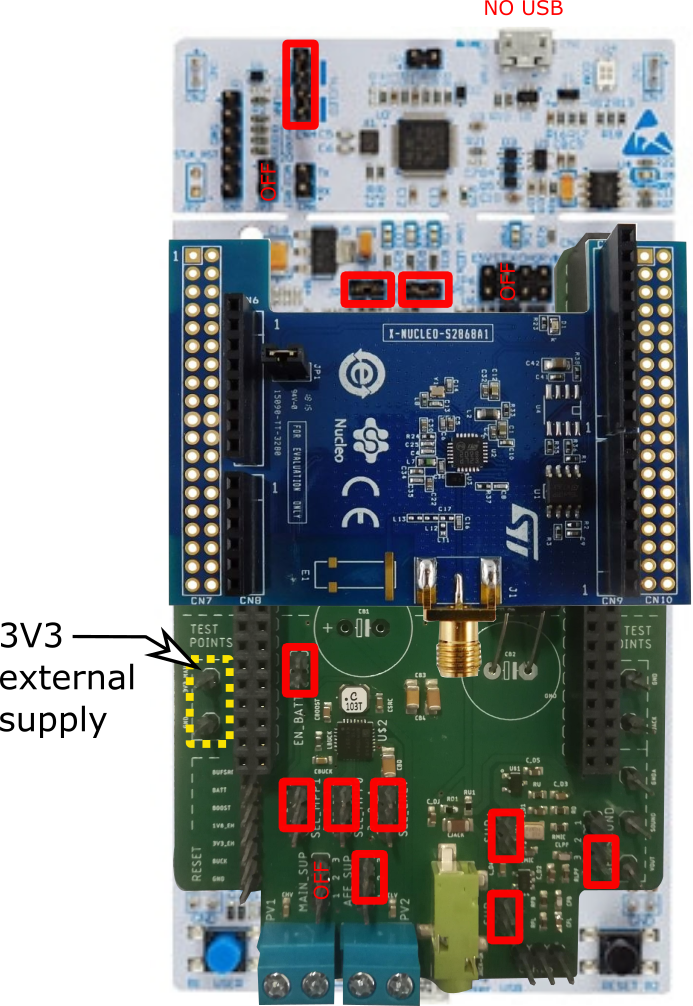
\includegraphics[width=0.5\textwidth]{figs/settings-mode-3V3.png}
    \caption{Settings for the boards, power monitoring mode.}
    \label{fig:settings-mode-3V3}
\end{figure}

%%%%%%%%%%%%%%%%%%%%%%%%%%%%%%%%%%%%%%%%%%%%%%%%%%%%%%%%%%%%%%%%%%%%%%%%%%%%%%%%%%%%
\clearpage
\subsection{Energy harvesting mode (EH): powered by PV cells} \label{sec:mode-EH}

This mode is the one that you will use to test your solution in real-world conditions: you can go full embedded by using energy harvesting of the environment thanks to the PV cells and harvesting circuitry. In this MODE, you also have a limited amount of functionalities: you cannot program the MCU anymore (or even debug it!) and you cannot receive data from the MCU through the UART interface either. Therefore, we recommend you to use this mode when (1) you have reached an advanced step of development i.e., stable and at least partially optimized; (2) you have tested in advance if your solution works in the \textit{Power monitoring mode}, see Section \ref{sec:mode-3V3}.

\textbf{In order not to damage the boards}, you need to make sure the following settings are properly set on your hardware:

\begin{itemize}
    \item First, make sure that all jumpers shown in red in Fig \ref{fig:settings-mode-eh} are configured as in the Figure.
   Be really careful for the OFF jumpers: these slots have to be open (with NO jumper). If you are not sure, please call use before powering the setting. It is always a better idea to ask a question rather than damaging the boards. There is nothing to set on the radio board.
    \item Then, plug in your PV cell(s) to harvest solar energy from the environment. Pay attention to the polarity.
    \item Finally, check out how your solution is behaving in real-life conditions!
\end{itemize}


\begin{bclogo}[couleur = gray!20, arrondi = 0.2, logo=\bcattention]{RESET procedure}
In this mode, you need to carry out a \textbf{RESET} procedure each time you want to change a setting. On the lower left part of the custom board, you have a RESET label and 7 pin headers. You need to connect each pin header to the GND pin header (the last one), starting from the first one (BUFSRC) to the sixth one (BUCK) as shown in Fig \ref{fig:reset-procedure}. Make sure you do not short two pin headers together when doing the reset procedure. Note that you can also use these pin headers to \textbf{monitor the signals} of the EH part of the board: this can be very useful, especially for the following signals: BATT, 3V3\_EH and 1V8\_EH.
\end{bclogo}

\begin{figure}[h!]
    \centering
    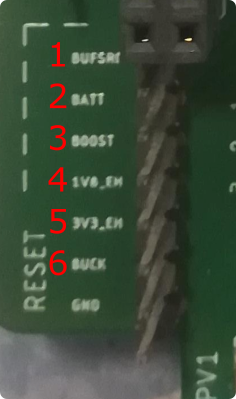
\includegraphics[width=0.15\textwidth]{figs/reset-procedure.png}
    \caption{RESET pin headers.}
    \label{fig:reset-procedure}
\end{figure}

\begin{figure}[h!]
    \centering
    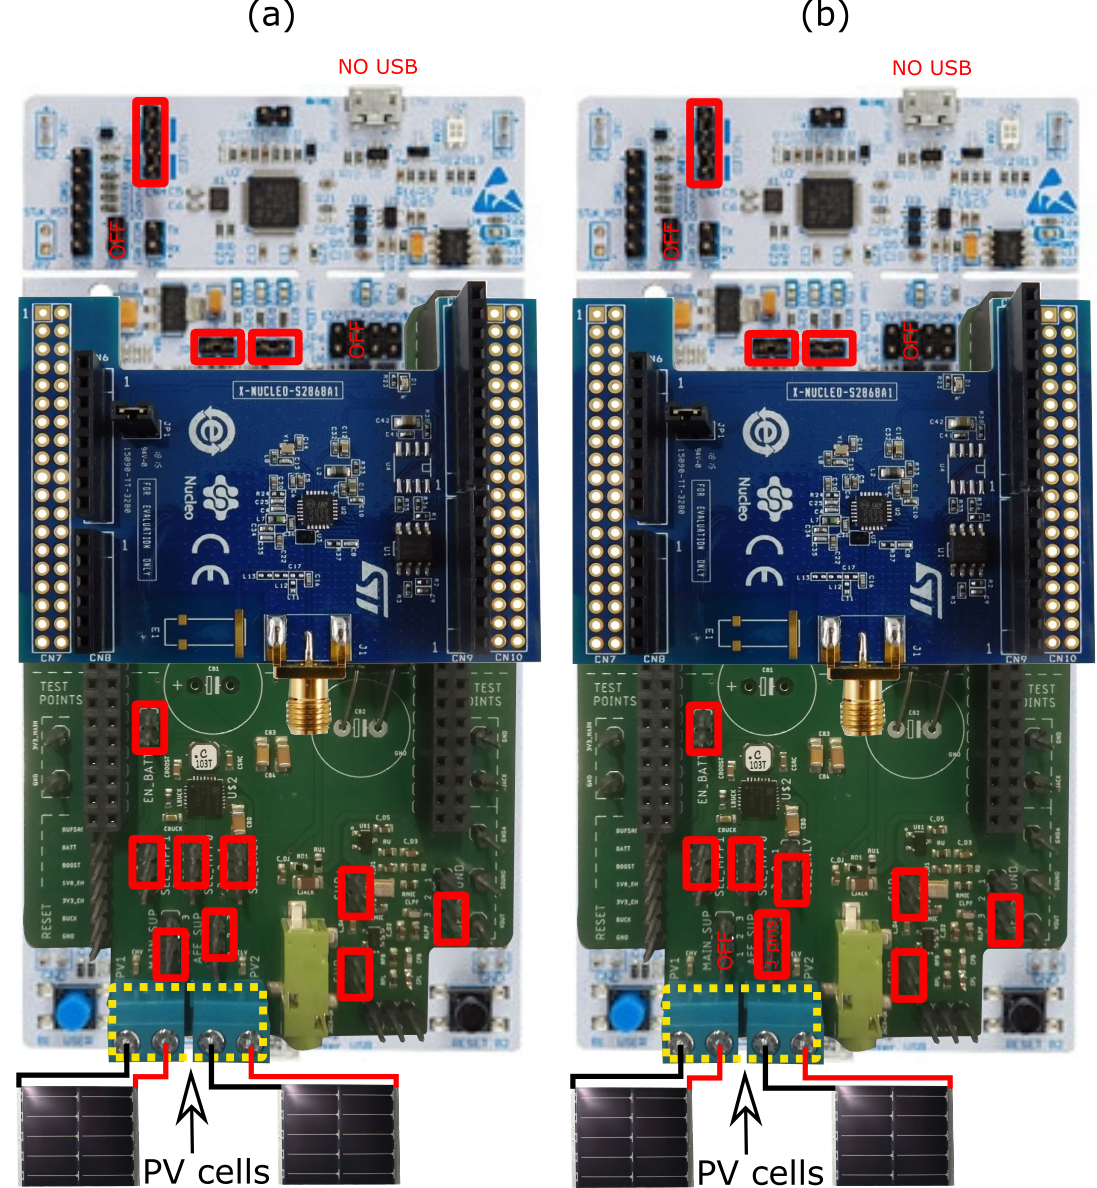
\includegraphics[width=0.7\textwidth]{figs/settings-mode-eh.png}
    \caption{Settings for the boards, EH mode. It is possible to supply all boards at once with (a) 3V3\_EH and (b) 1V8\_EH. Be careful to set properly all jumpers.}
    \label{fig:settings-mode-eh}
\end{figure}

\begin{bclogo}[couleur = gray!20, arrondi = 0.2, logo=\bcinfo]{Supplying the system at 1V8 with EH}
You can enable the 1V8 LDO output from the energy harvesting chip by changing the jumper SEL\_ENLV as presented in Table \ref{tab:EH-headers}. You can then chose to supply the whole system with that 1V8 source. To do this, make sure the MAIN\_SUP jumper is OFF and then, use a 3-pins jumper that we can provide you (on demand!) to connect the 3 pins of the AFE\_SUP together, as shown in Fig. \ref{fig:settings-mode-eh}b. \textbf{Important}: do not put anything else than the PV cells in the blue connectors !
\end{bclogo}

\clearpage
\section{Testing procedures} \label{sec:test}

The purpose of this testing procedure is to verify that the custom board you have received is fully functional. They have all been already tested once but this is a good occasion for you to get your hands into the hardware for the first time! If you have any issue later on, start by re-doing this procedure and if it does not work, contact us to start the debugging together.

\subsection{Basic functionalities}

Please make sure you carry out this procedure the first time you get your boards.

\begin{itemize}
    \item Set the boards in \textit{Development mode}, see Section \ref{sec:mode-dev}.
    \item Make sure the "PWR LED" is ON.
    \item Make sure the AFE part is supplied (by connecting jumpers SUP+ and SUP-).
    \item Connect an oscilloscope to monitor the 3V3\_MAIN signal and the SOUND signal.
    \item Connect your PC audio through the mini-jack input on the board.
    \item Use a jumper to connect SEL\_SOUND to 1 (JACK): you should see the signal clearly on the oscilloscope (make sure the sound level on your computer is high enough). The signal should be centered around 1.65 V.
    \item Finally, move the jumper to connect SEL\_SOUND to 3 (AFE). Clap in your hands or say something: you should see it clearly on the oscilloscope (1V scale). The signal should be centered around 1.65 V.
    \item If you got here without any issue, the basic functionalities of the power-management board are working properly. Note that the EH part of the power-management board is not covered here.
\end{itemize}


\subsection{EH circuit only}

\begin{itemize}
    \item Set the boards as presented in Fig. \ref{fig:testing-mode-eh}.
    \item Connect an oscilloscope to monitor the signals highlighted with a purple star in Fig. \ref{fig:testing-mode-eh}. Nothing should happen if no PV cell is connected.
    \item Then, connect one PV cell (and double-check the polarity!). You can connect two PV cells but it is not necessary.
    \item You should see the BATT signal rising as energy is harvested from the environment thanks to the harvesting circuit and stored in the capacitor (C = 1 mF). When the BATT signal reaches a specific value (check out the AEM10941 datasheet!), it switches on the EH outputs i.e., 3V3\_EH and 1V8\_EH. Can you see that ?
    \item If the AFE part is supplied (jumpers SUP+ and SUP- connected), it should slowly draw energy from the capacitor.
    \item Make sure that SEL\_SOUND is connected to 3 (AFE). Clap in your hands or say something: you should see it clearly on the oscilloscope. Note: you could also power the AFE with the 3V3\_EH if you want but you need to make sure you connect the right pins: please ask support if you are not 100\% sure how to do it !
    \item If you got here without any issue, it means that the EH part of your power-management board seems to work properly.
\end{itemize}

\begin{figure}[h!]
    \centering
    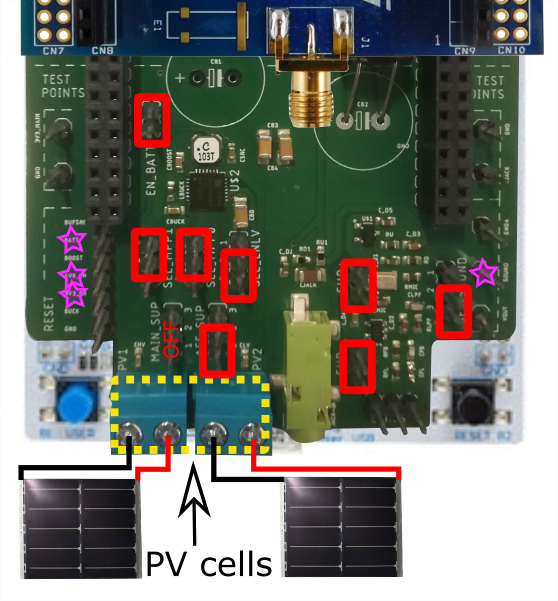
\includegraphics[width=0.5\textwidth]{figs/testing-EH.png}
    \caption{Specific settings for the power management board in order to test the EH circuit. Other jumpers must be set as shown in Fig. \ref{fig:settings-mode-eh}.}
    \label{fig:testing-mode-eh}
\end{figure}

\vspace{0.5cm}
\flushright
That's all folks !


\end{document}

%%%%%%%%%%%%%%%%%%%%%%%%%%%%%%%%%%%%%%%%%%%%%%%%%%%%%%%%%%%%%%%%%%%%%%%%%%%%
